%%%%%%%%%%%%%%%%%%%%%%%%%%%%%%%%%%%%%%%%%
% Beamer Presentation
% LaTeX Template
% Version 1.0 (10/11/12)
%
% This template has been downloaded from:
% http://www.LaTeXTemplates.com
%
% License:
% CC BY-NC-SA 3.0 (http://creativecommons.org/licenses/by-nc-sa/3.0/)
%
%%%%%%%%%%%%%%%%%%%%%%%%%%%%%%%%%%%%%%%%%

%----------------------------------------------------------------------------------------
%	PACKAGES AND THEMES
%----------------------------------------------------------------------------------------

\documentclass{beamer}



\mode<presentation> {



% The Beamer class comes with a number of default slide themes
% which change the colors and layouts of slides. Below this is a list
% of all the themes, uncomment each in turn to see what they look like.

%\usetheme{default}
%\usetheme{AnnArbor}
%\usetheme{Antibes}
%\usetheme{Bergen}
%\usetheme{Berkeley}
%\usetheme{Berlin}
%\usetheme{Boadilla}
%\usetheme{CambridgeUS}
%\usetheme{Copenhagen}
%\usetheme{Darmstadt}
%\usetheme{Dresden}
%\usetheme{Frankfurt}
%\usetheme{Goettingen}
%\usetheme{Hannover}
%\usetheme{Ilmenau}
%\usetheme{JuanLesPins}
%\usetheme{Luebeck}
\usetheme{Madrid}
%\usetheme{Malmoe}
%\usetheme{Marburg}
%\usetheme{Montpellier}
%\usetheme{PaloAlto}
%\usetheme{Pittsburgh}
%\usetheme{Rochester}
%\usetheme{Singapore}
%\usetheme{Szeged}
%\usetheme{Warsaw}

% As well as themes, the Beamer class has a number of color themes
% for any slide theme. Uncomment each of these in turn to see how it
% changes the colors of your current slide theme.

%\usecolortheme{albatross}
%\usecolortheme{beaver}
%\usecolortheme{beetle}
%\usecolortheme{crane}
%\usecolortheme{dolphin}
%\usecolortheme{dove}
%\usecolortheme{fly}
%\usecolortheme{lily}
%\usecolortheme{orchid}
%\usecolortheme{rose}
%\usecolortheme{seagull}
%\usecolortheme{seahorse}
%\usecolortheme{whale}
%\usecolortheme{wolverine}

%\setbeamertemplate{footline} % To remove the footer line in all slides uncomment this line
%\setbeamertemplate{footline}[page number] % To replace the footer line in all slides with a simple slide count uncomment this line

%\setbeamertemplate{navigation symbols}{} % To remove the navigation symbols from the bottom of all slides uncomment this line

\usepackage{tikz}
\usepackage{setspace}

\usepackage{siunitx}
%\usetheme{Madrid}
\useoutertheme{miniframes} % Alternatively: miniframes, infolines, split
\useinnertheme{circles}
\beamertemplatenavigationsymbolsempty

%\definecolor{UBCblue}{rgb}{0.04706, 0.13725, 0.26667} % UBC Blue (primary)
%\definecolor{UBCgrey}{rgb}{0.3686, 0.5255, 0.6235} % UBC Grey (secondary)
%%\definecolor{crcgreen}{rgb}{116/255, 198/255, 155/255}
%\definecolor{crcgreen}{rgb}{0.454, 0.776, 0.608}
%\setbeamercolor{palette primary}{bg=white,fg=crcgreen}
%\setbeamercolor{palette secondary}{bg=white,fg=white}
%\setbeamercolor{palette tertiary}{bg=white,fg=white}
%\setbeamercolor{palette quaternary}{bg=white,fg=white}
%\setbeamercolor{structure}{fg=white} % itemize, enumerate, etc
%\setbeamercolor{section in toc}{fg=white} % TOC sections
%
%% Override palette coloring with secondary
%\setbeamercolor{subsection in head/foot}{bg=white,fg=white}






}

\date{12th International Conference on Urban Climate (ICUC12), Rotterdam, The Netherlands, 7–11 Jul 2025}
\usepackage{bibentry}
\nobibliography*
\usepackage{multicol}
%\usepackage{ulem}
\usepackage{graphicx} % Allows including images
%\usepackage{booktabs} % Allows the use of \toprule, \midrule and \bottomrule in tables
\usepackage[sort&compress,square,comma,authoryear]{natbib}
\bibliographystyle{plainnat}
%\bibliographystyle{kerry_harvard}
\renewcommand\bibfont{\scriptsize}

 \newcommand\makebeamertitle{\frame{\maketitle}}%
 
 \beamertemplatenavigationsymbolsempty
 \setbeamertemplate{headline}{}

%----------------------------------------------------------------------------------------
%	TITLE PAGE
%----------------------------------------------------------------------------------------



\begin{document}


%\title[The SIMPEL soil water balance module]{Improving urban water process representations in land surface models with the SIMPEL soil water balance module}
%\author[Nice, KA et al.]
%{Kerry A. Nice$^{1}$, Harro J. Jongen$^{2}$, Kristian Förster$^{3}$
%}
%\institute[UoM]{{\begin{flushleft}
%\tiny $^{1}$Transport, Health, and Urban Systems Research Lab, Faculty of Architecture, Building and Planning, University of Melbourne.\\$^{2}$Institute for Water and Environment, Karlsruhe Institute of Technology, Karlsruhe, Germany.\\$^{3}$Institute of Ecology and Landscape, Department of Landscape Architecture, Hochschule Weihenstephan-Triesdorf, Freising, Germany.
%\end{flushleft}}}
%\titlegraphic{
\includegraphics[scale=0.75]{template_icuc12_logo.png}~~~~
\includegraphics[scale=0.5]{image001.jpg}~~~
\includegraphics[scale=0.10]{karlsruhe-institute-of-technology-kit-logo-png_seeklogo-353008_.png}~~~
\includegraphics[scale=0.12]{Hochschule_Weihenstephan-Triesdorf_Logo.svg.png}}
%\makebeamertitle



{
\usebackgroundtemplate{%
\tikz\node[opacity=0.2,inner sep=0] {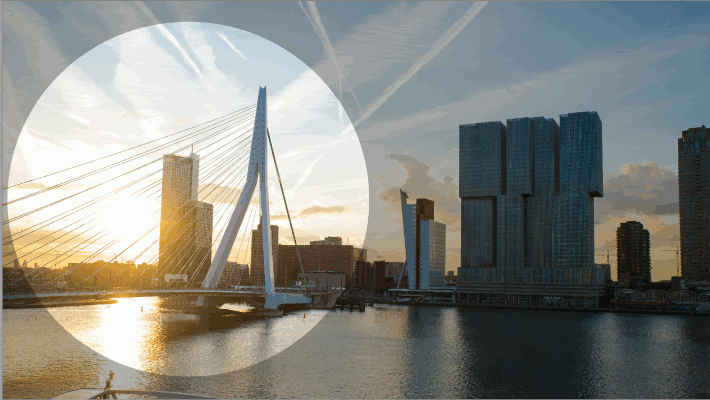
\includegraphics[height=\paperheight,width=\paperwidth]{Screenshot_20250702_152356_scale.png}};}

\title[The SIMPEL soil water balance module]{Improving urban water process representations in land surface models with the SIMPEL soil water balance module}
\author[Nice, KA et al.]
{Kerry A. Nice$^{1}$, Harro J. Jongen$^{2}$, Kristian Förster$^{3}$
}
\institute[UoM]{{\begin{flushleft}
\tiny $^{1}$Transport, Health, and Urban Systems Research Lab, Faculty of Architecture, Building and Planning, University of Melbourne.\\$^{2}$Institute for Water and Environment, Karlsruhe Institute of Technology, Karlsruhe, Germany.\\$^{3}$Institute of Ecology and Landscape, Department of Landscape Architecture, Hochschule Weihenstephan-Triesdorf, Freising, Germany.
\end{flushleft}}}
\titlegraphic{
\includegraphics[scale=0.75]{template_icuc12_logo.png}~~~~
\includegraphics[scale=0.5]{image001.jpg}~~~
\includegraphics[scale=0.10]{karlsruhe-institute-of-technology-kit-logo-png_seeklogo-353008_.png}~~~
\includegraphics[scale=0.12]{Hochschule_Weihenstephan-Triesdorf_Logo.svg.png}}
\makebeamertitle
}





\begin{frame}{Motivation: Modelling irrigation} 

\begin{itemize}
\item Irrigation trials at University of Melbourne (Burnley)$^{1}$. Looking for model capable of reproducing micro-scaled results.\\ 
\item But most hydrology models are at a catchment scale.
\end{itemize}
\begin{center}
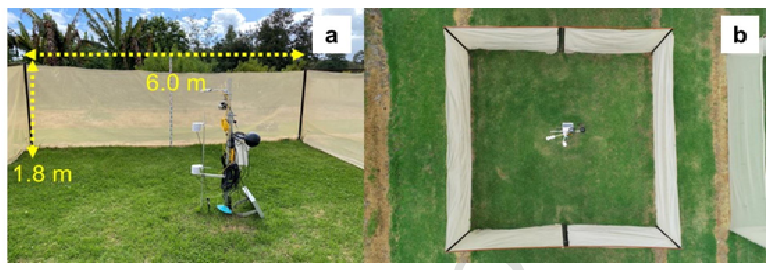
\includegraphics[scale=0.60]{Screenshot_20250703_100546.png}
\end{center}
$^{1}${\footnotesize \cite{Cheung2024} (paper), 10.5281/zenodo.10140668, 10.5281/zenodo.10972538 (datasets)}
\end{frame}






\begin{frame}{Motivation: Urban Plumber} 
\begin{itemize}

\item Meanwhile, Urban Plumber results: most urban models do a terrible job with hydrology {\footnotesize \citep{jongen_water_2024}}.
\begin{itemize}
\item Most don't account for hydrology at all
\item If they do, water budget rarely closed
\item Or fully account for all types of indicators (runoff, infiltration, ET, storage)
\item Leading to less accurate modelling
\end{itemize}
\item Urban Plumber and previous intercomparisions: Latent energy fluxes in urban areas poorly predicted by most models {\footnotesize \citep{lipson_evaluation_2024,grimmond_initial_2011}}
\item This is also true of my models, TARGET and VTUF-3D \citep{Nice2018}
\end{itemize}
\end{frame}









\begin{frame}{The SIMPEL model} 


\begin{columns}

\begin{column}{0.5\textwidth}
\begin{itemize}
\item Single bucket model
\item Original Excel spreadsheet developed by Georg Hörmann
\item Extended (snow, surface runoff) by Kristian Förster 2022
\item Adapted by Kerry Nice 2023-5
\item Added support for hourly timesteps, irrigation, additional site specific parameters
\end{itemize}
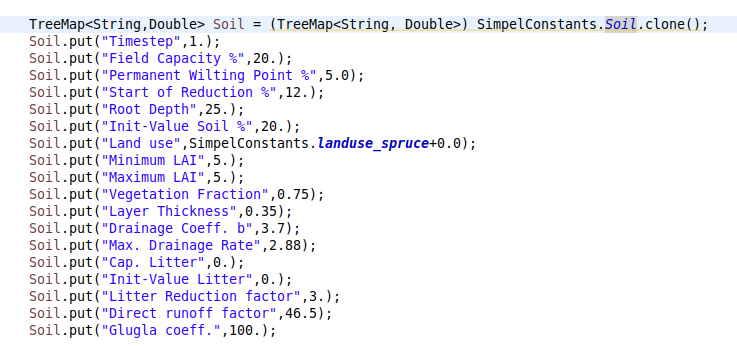
\includegraphics[scale=0.33]{Screenshot_20250703_140316.png}
\end{column}

\begin{column}{0.5\textwidth}
 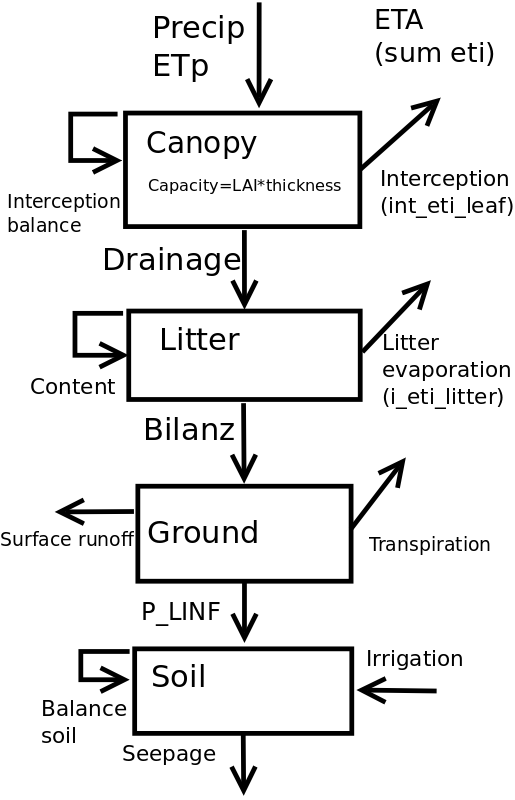
\includegraphics[scale=0.30]{Simpel_diagram2.png}\\
{\scriptsize Adapted from \cite{hormann_comparison_2007}}
\end{column}

\end{columns}




\end{frame}





\begin{frame}{Validations against Burnley irrigation observations} 
\begin{center}
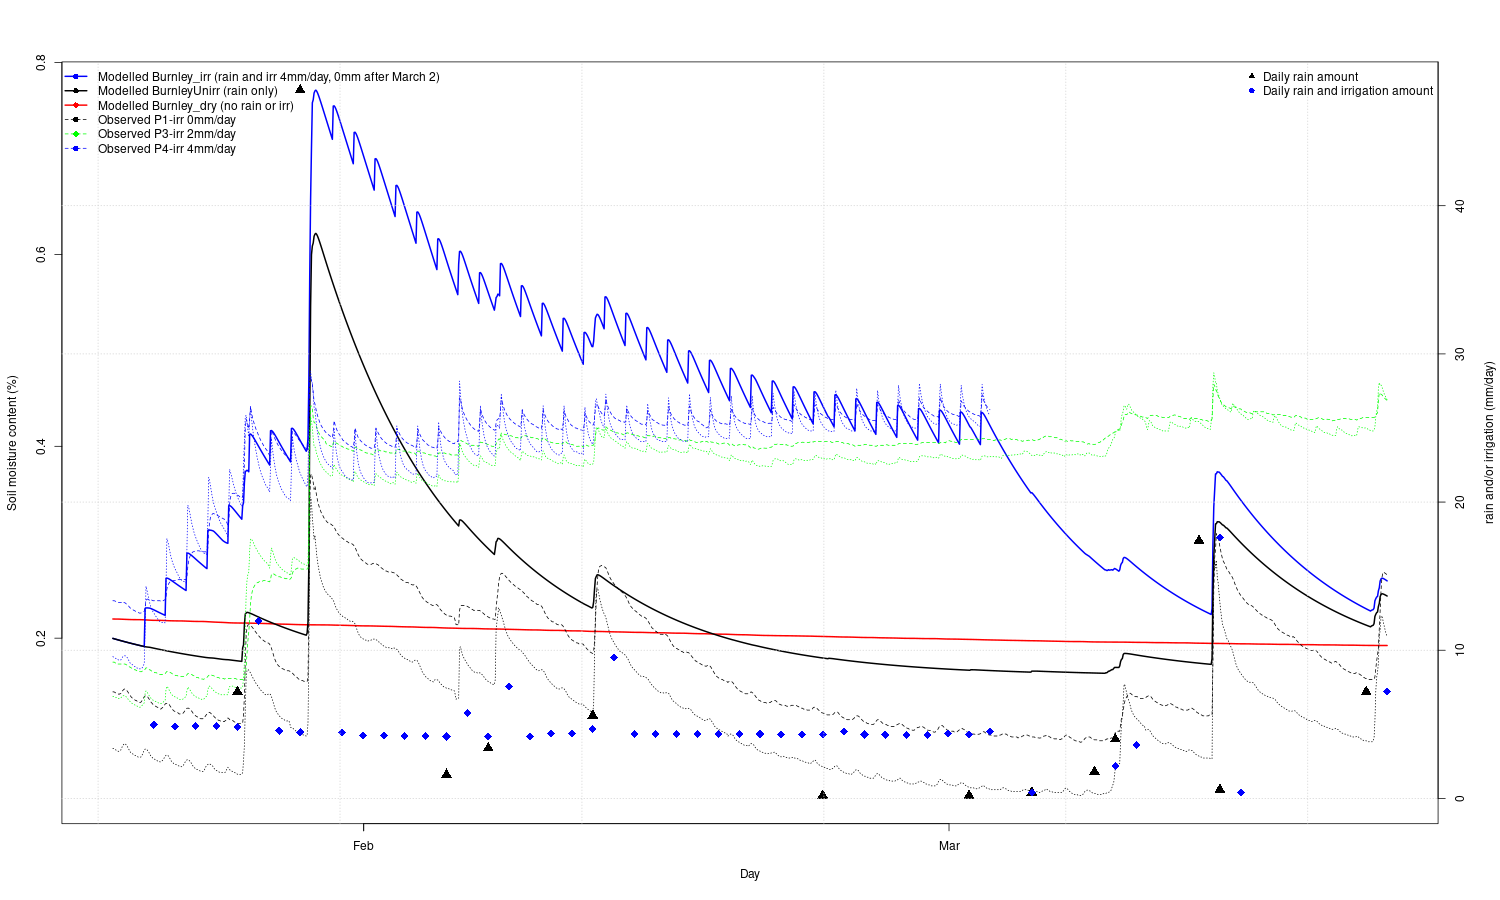
\includegraphics[scale=0.18]{BurnleyComparisons.png}
\end{center}

Initial testing of SIMPEL model with Burnley observations$^{1}$ were promising. Reproducing soil moisture of different irrigation amounts (0, 2, 4mm/day).
\\
$^{1}${\tiny \cite{Cheung2024}, 10.5281/zenodo.10140668, 10.5281/zenodo.10972538}
\end{frame}



\begin{frame}{The SIMPEL evaporotranspiration comparisons with Urban Plumber sites} 

{\footnotesize And broad agreement across many Urban Plumber sites of evaporotranspiration levels}
\begin{center}
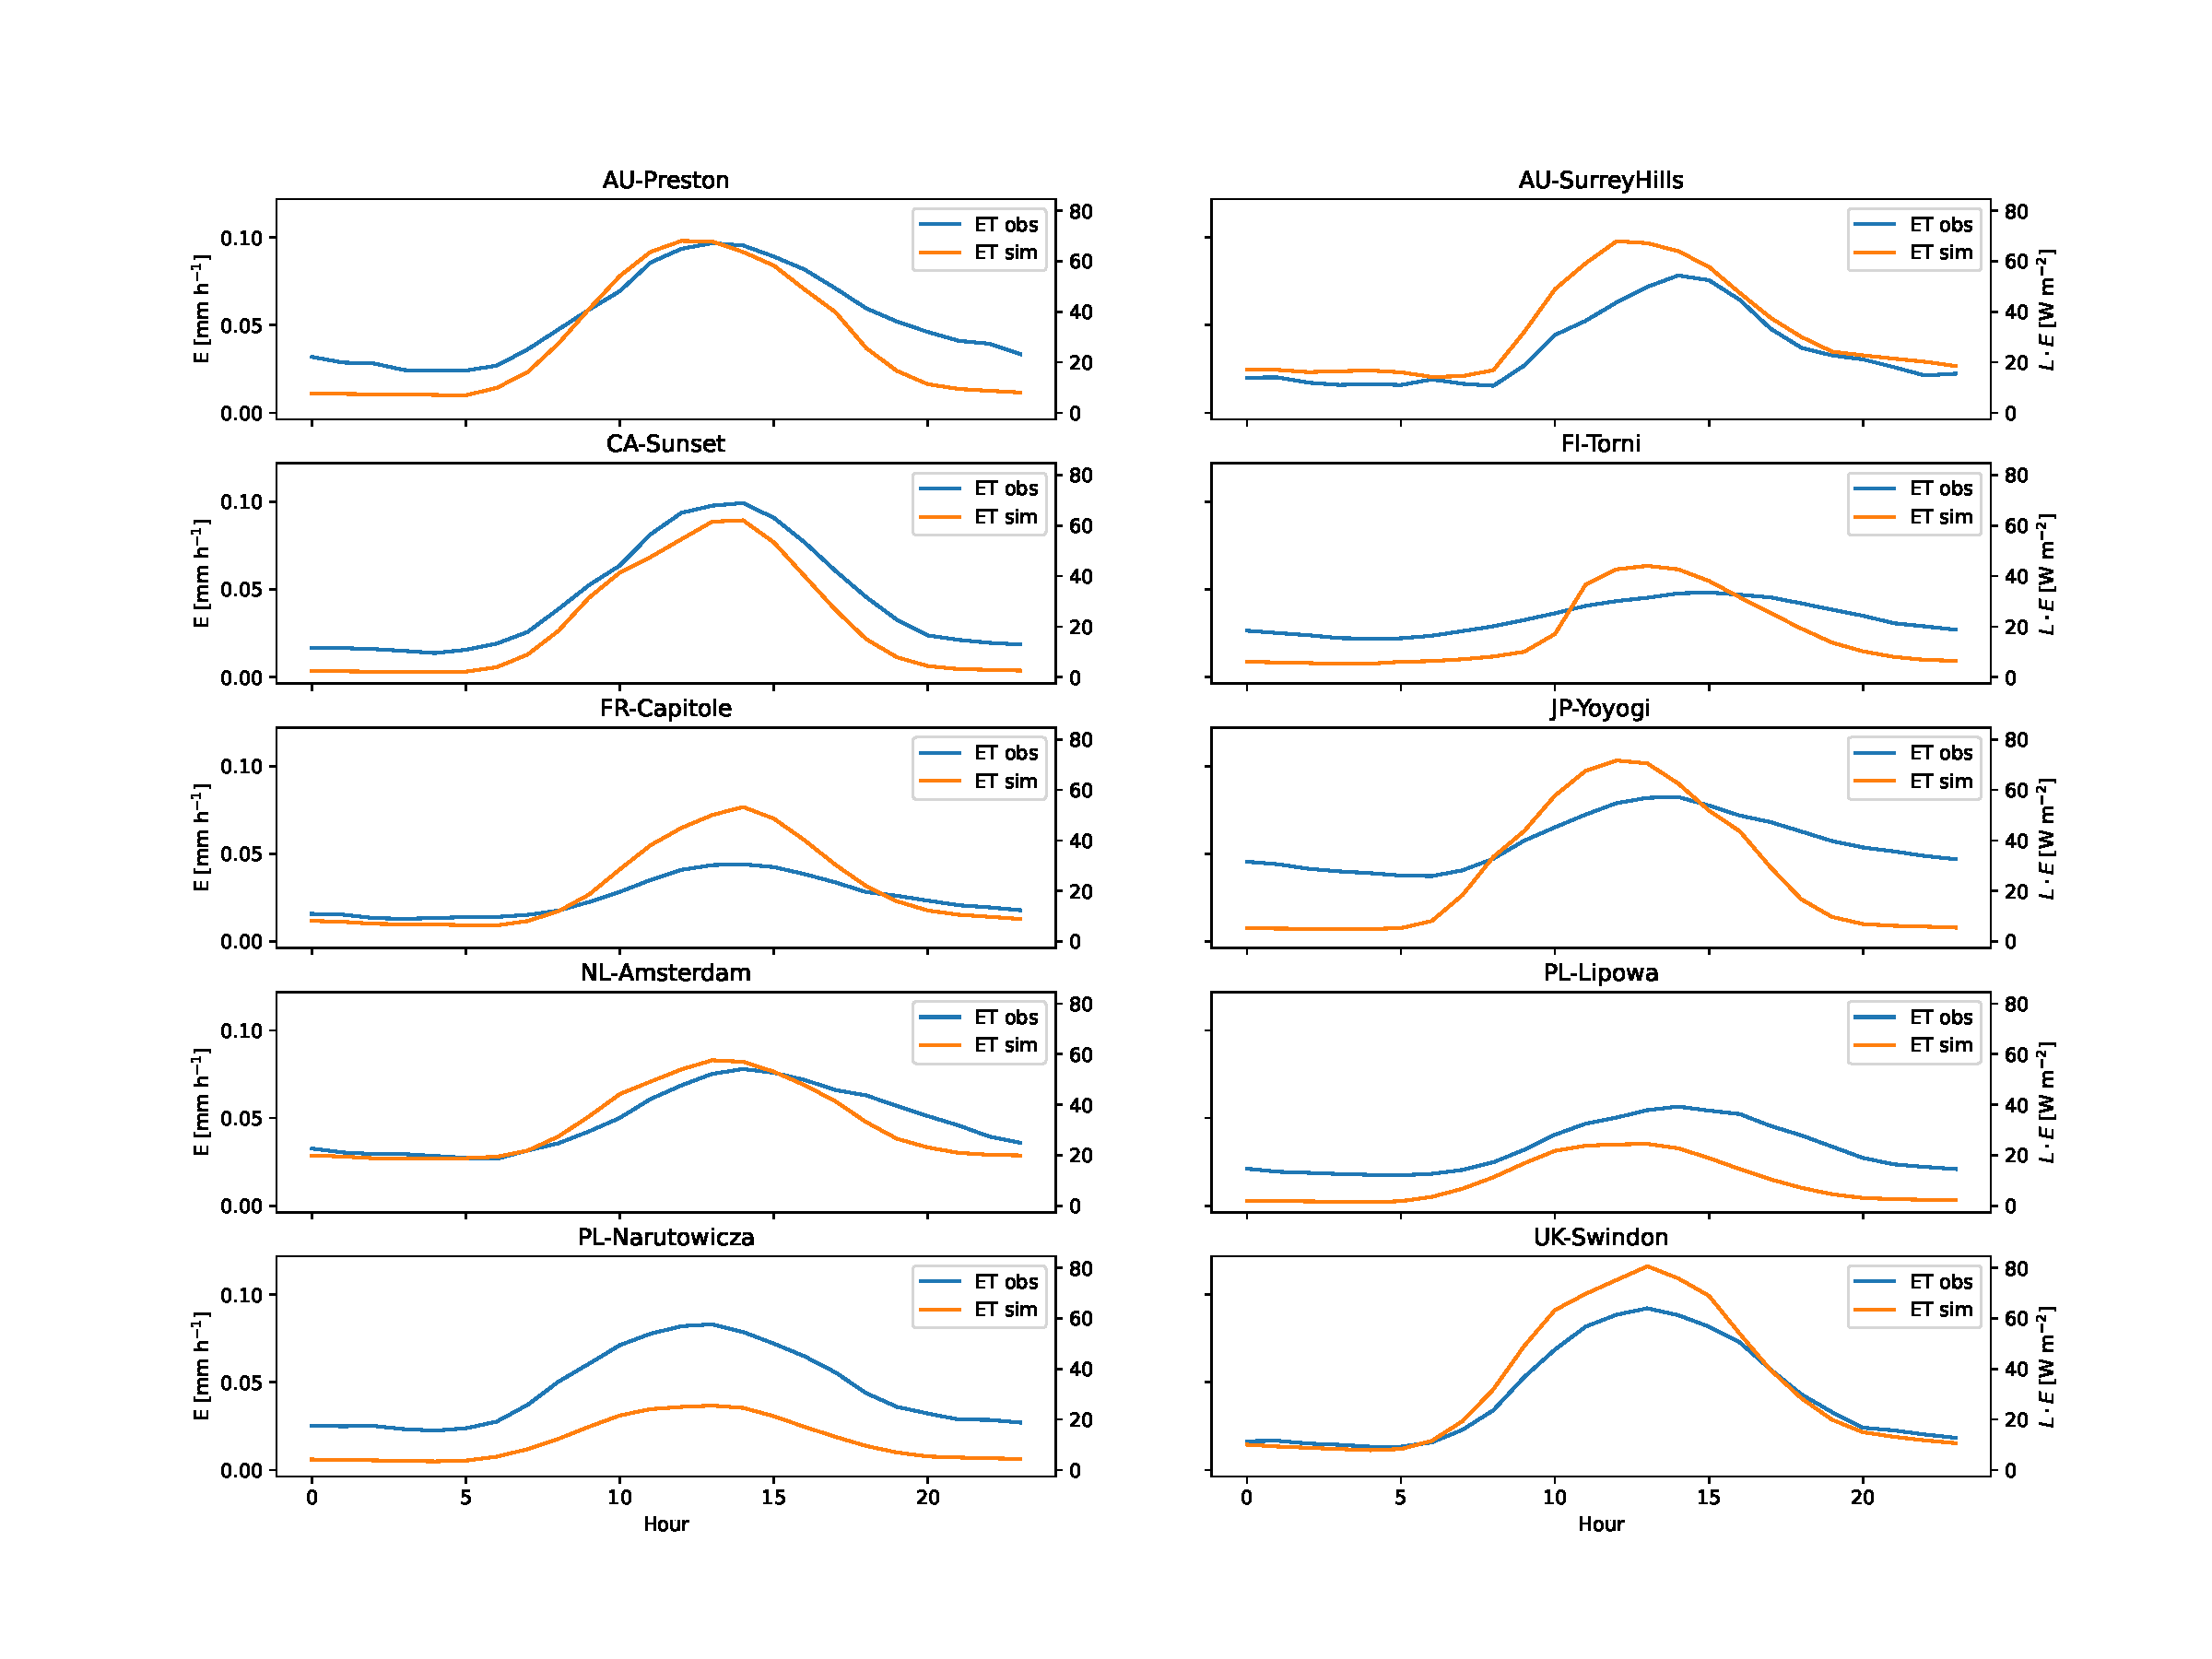
\includegraphics[scale=0.24]{et_presunangle.pdf}
\end{center}
\end{frame}



\begin{frame}{The SIMPEL water balance comparisons with Urban Plumber sites} 
And includes necessary components for water balance closure
\begin{center}
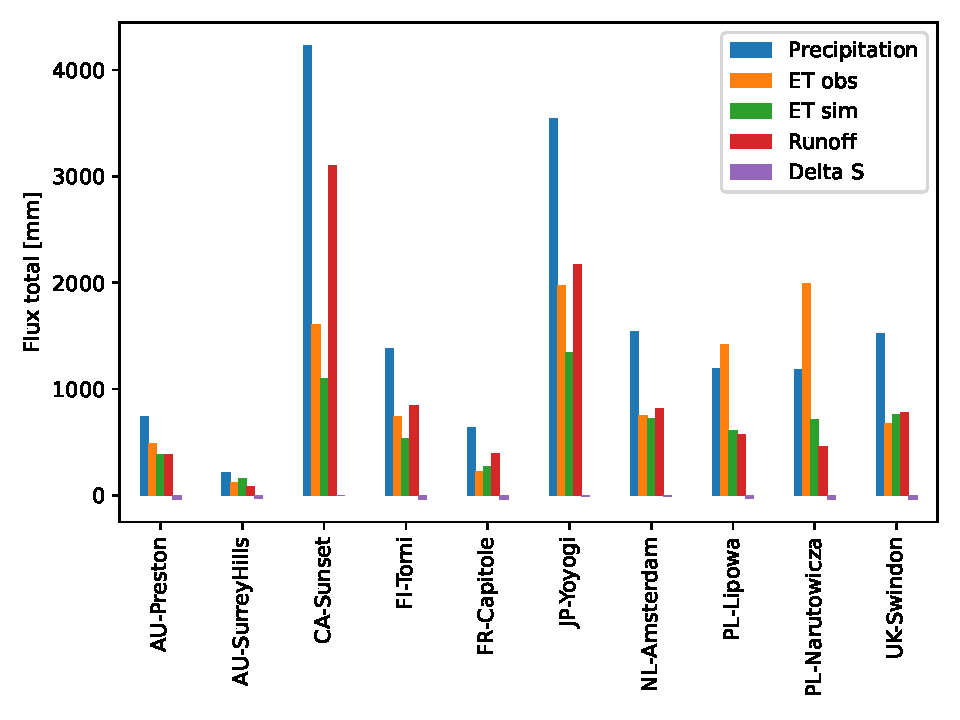
\includegraphics[scale=0.50]{water_balance_presunangle.pdf}
\end{center}
\end{frame}



\begin{frame}{Integration into TARGET} 

\begin{center}
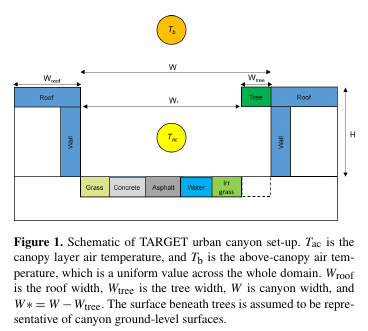
\includegraphics[scale=0.60,trim={20 80 20 10},clip]{TARGET1.png}
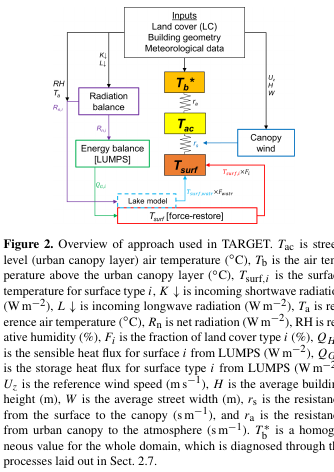
\includegraphics[scale=0.60,trim={20 180 20 0},clip]{TARGET2.png}
\end{center}
The Air-temperature Response to Green/blue-infrastructure Evaluation Tool (TARGET) is a computationally efficient model designed to evaluate blue/green infrastructure, based on an urban canyon and aggregations of different land cover types \citep{Broadbent2019}.
\end{frame}


\begin{frame}{Integration into TARGET} 

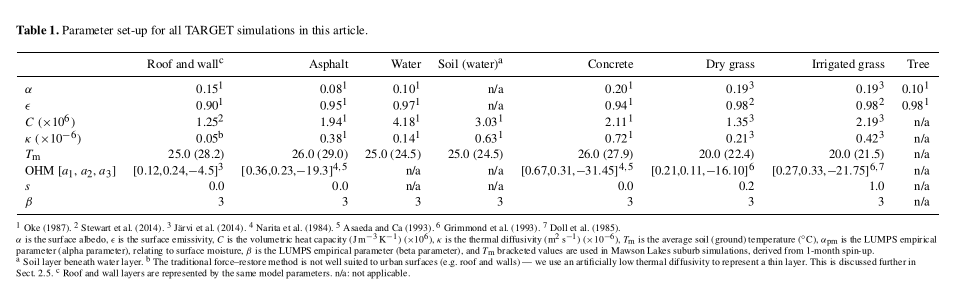
\includegraphics[scale=0.45]{TARGET3.png}

\begin{itemize}
\item Hydrology was not previously included
\item Latent energy was indirectly calculated from ground flux heat storage calculations for different surface types using the $\alpha$ coefficient of the OHM model
\item SIMPEL allows replacement with hydrologically based evaporotranspiration and latent energy calculations requiring very minor additional computational costs.
\item Provides additional capability to account for irrigation, drought and other hydrological impacts
\end{itemize}
\end{frame}


\begin{frame}{TARGET evaluation against Preston observations} 

{\footnotesize At this early stage of development, TARGET provides reasonable agreement with observed latent energy (top panel) of Urban Plumber Preston site \citep{Coutts2007}.}
\\
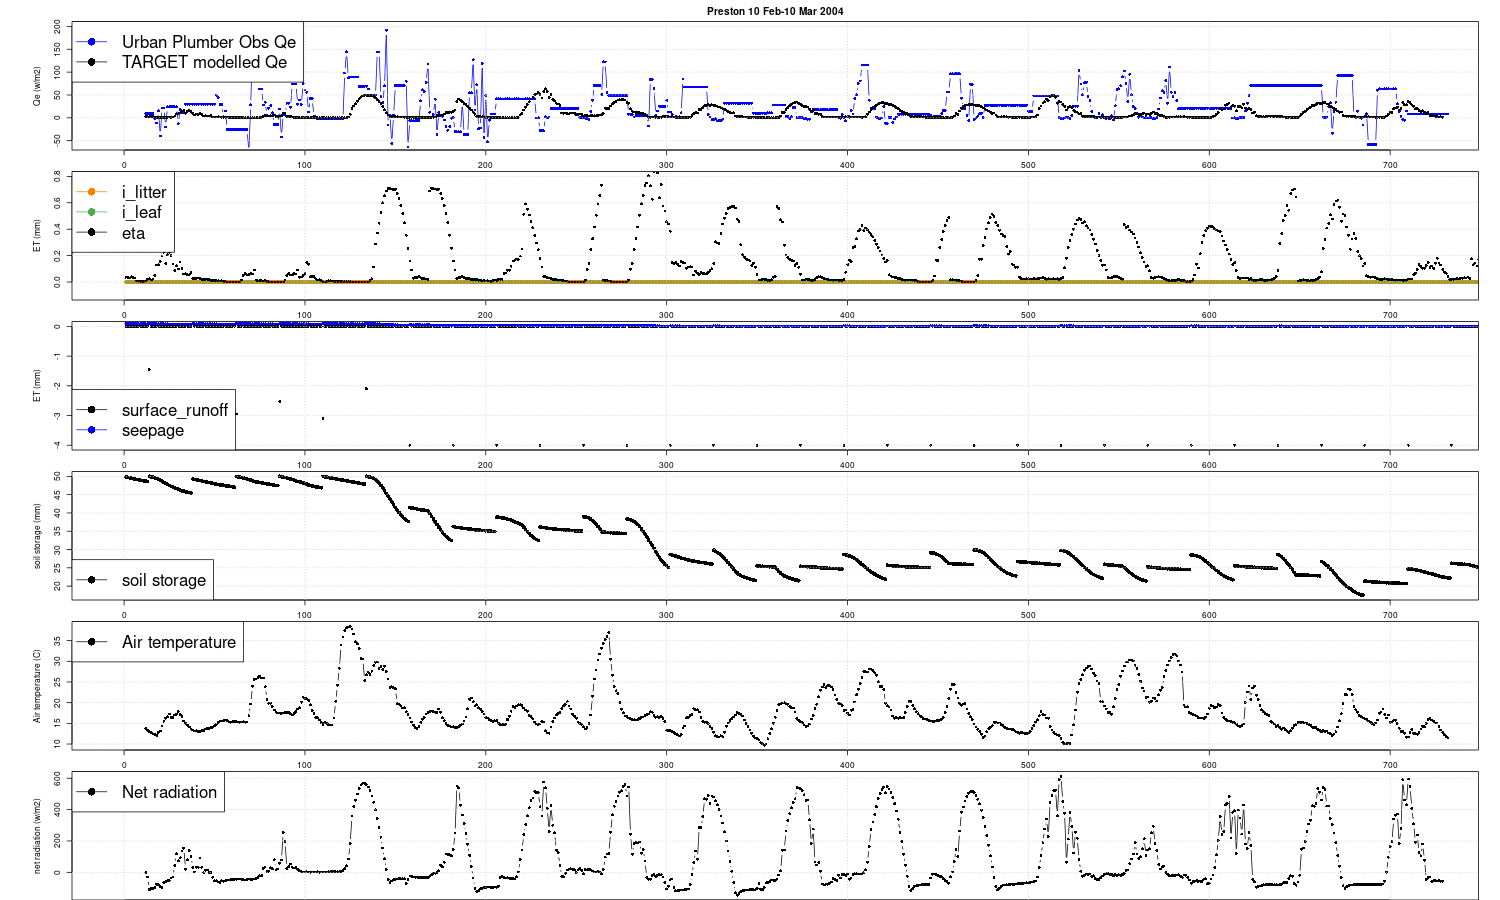
\includegraphics[scale=0.20]{PrestonFeb2004_4mmIrr_ground.png}
\end{frame}


\begin{frame}{Future plans} 

\begin{itemize}

\item Integration into TARGET as a single surface type (irrigated grass) is nearly complete:

\item Integration into VTUF-3D as gridded individual patches of pervious/vegetated surfaces and underlying soil is in progress: 

\item Improvement of ET using stomatal models to incorporate additional vegetation types

\item Tuning and testing the model across a range of climate zones and city types

\item SIMPEL model could also be integrated into other urban models, providing micro-scaled hydrology for a variety of vegetated and pervious surface types:

\item Or more accurate runoff for impervious surfaces

\item Integration with UMEP plugin version of TARGET (come to the UMEP workshop on Thursday afternoon)

\end{itemize}

\begin{itemize}
\setlength\itemsep{-0.55em}
\item[] {\tiny https://github.com/mothlight/Target-Java.v2}
\item[] {\tiny https://github.com/mothlight/VTUF-3D-Java.v2/} 
\item[] {\tiny https://github.com/mothlight/Simpel} 
\item[] {\tiny https://umep-docs.readthedocs.io/en/latest/processor/Urban\%20Heat\%20Island\%20TARGET.html}
\end{itemize}

\end{frame}




%\begin{frame}<presentation:0>[noframenumbering]
%\begin{frame}[allowframebreaks]
\begin{frame}[shrink=25]{References}
\begin{multicols}{2}
\section*{References}
%\bibliographystyle{kerry_harvard}
%\nocite{*}
%\bibliographystyle{plain}
\bibliography{library}
\end{multicols}
\end{frame}

\begin{frame}{Thank you}
\begin{center}
\textbf{Dr Kerry Nice} 

Transport, Health, and Urban Systems Research Lab\\ Faculty of Architecture, Building and Planning\\ University of Melbourne



https://mothlight.github.io/
\\
~
\\

\includegraphics[scale=0.02,trim = 0mm 0mm 0mm 0mm, clip]{207_Mastodon_logo_logos-512.png} @mothlight@fediscience.org
\\
~
\\

\includegraphics[scale=0.75,trim = 0mm 0mm 0mm 0mm, clip]{Logo2.png}
\end{center} 
\end{frame}

\end{document}
